\begin{figure}[t]
\centering
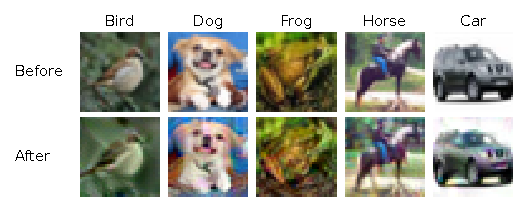
\includegraphics[width=\columnwidth]{ablations/figures/mipa_components_cifar10/paper_examples.pdf}
\par\vspace{2pt}
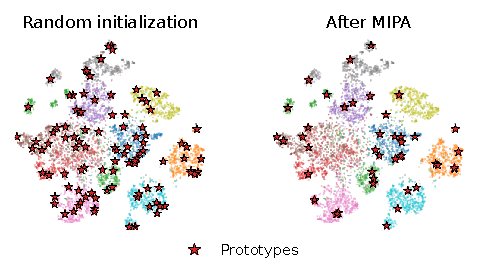
\includegraphics[width=\columnwidth]{ablations/figures/mipa_components_cifar10/prototype_tsne.pdf}
\caption{CIFAR10 prototypes before and after MIPA at 0.2\% size. Top: five selected illustrative prototype pairs from five original-image classes, before optimization and after 10k iterations. Each column tracks the same prototype; pixels are displayed without enhancement. Bottom: one joint t-SNE of 10,000 randomly sampled real-image features and all 100 initial and final prototypes, using the frozen teacher. Both t-SNE panels share coordinates and axis limits. Class labels are used only for selecting and annotating examples and coloring real images in the visualization; stars denote prototypes. The projection illustrates feature geometry rather than proving coverage or absence of collapse.}
\label{fig:mipa-qualitative}
\end{figure}
